%%%%%%%%%%%%%%%%%%%%%%%%%%%%%%%%%%%%%%%%%%%%%%%%%%%%%%%%%%%%%%%%%%%%%%%%%%%%%%%%%%
\begin{frame}[fragile]\frametitle{}
\begin{center}
{\Large Introduction to Indian Philosophy (Darshana)}
\end{center}
\end{frame}

%%%%%%%%%%%%%%%%%%%%%%%%%%%%%%%%%%%%%%%%%%%%%%%%%%%%%%%%%%%%%%%%%%%%%%%%%%%%%%%%%%
\begin{frame}[fragile]\frametitle{Indian Philosophy: The Darshanas}
\begin{columns}
\begin{column}{0.5\textwidth}
\begin{itemize}
\item The Darshanas are the six major philosophical schools of Hindu thought
\item They include Nyāya, Vaiśeṣika, Sāṃkhya, Yoga, Mīmāṃsā, and Vedānta
\item Each Darshana has its own unique perspective on the nature of reality, knowledge, and the ultimate goal of human existence
\item The Darshanas provide a rich and diverse intellectual framework for understanding the complexities of the Indian philosophical tradition
\item They have had a profound influence on the development of Indian religious, ethical, and social thought
\end{itemize}
\end{column}
\begin{column}{0.5\textwidth}
\begin{figure}
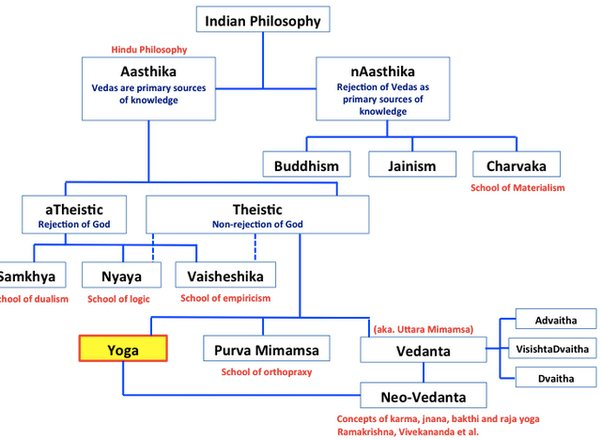
\includegraphics[width=\linewidth]{darshanas.jpg}
\caption{Indian Philosophy: Genesis and Various Schools of Thoughts - Indian Intellectual Tradition - Quora}
\end{figure}
\end{column}
\end{columns}
\end{frame}

%%%%%%%%%%%%%%%%%%%%%%%%%%%%%%%%%%%%%%%%%%%%%%%%%%%%%%%%%%%%%%%%%%%%%%%%%%%%%%%%%%
\begin{frame}[fragile]\frametitle{Hinduism}
\begin{columns}
\begin{column}{0.5\textwidth}
\begin{itemize}
    \item Hinduism is the oldest and most widely practiced religion in India
    \item Based on the Vedas, Upanishads, and other sacred texts
    \item Believes in Brahman as the ultimate reality and the divine self (Atman)
    \item Emphasizes the cycle of birth, death, and rebirth (samsara)
    \item Promotes the four main goals of life: dharma, artha, kama, and moksha
\end{itemize}
\end{column}
\begin{column}{0.5\textwidth}
\begin{figure}
    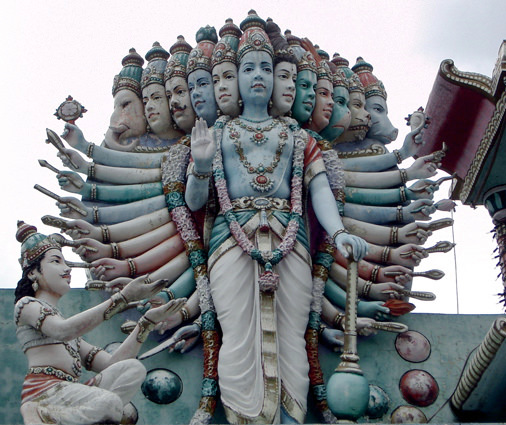
\includegraphics[width=\linewidth]{hinduism.jpg}
    \caption{Hinduism - World History Encyclopedia}
\end{figure}
\end{column}
\end{columns}
\end{frame}

%%%%%%%%%%%%%%%%%%%%%%%%%%%%%%%%%%%%%%%%%%%%%%%%%%%%%%%%%%%%%%%%%%%%%%%%%%%%%%%%%%
\begin{frame}[fragile]\frametitle{Buddhism}
\begin{columns}
\begin{column}{0.5\textwidth}
\begin{itemize}
    \item Buddhism was founded by Gautama Buddha in the 6th century BCE
    \item Emphasizes the Four Noble Truths and the Eightfold Path to end suffering
    \item Believes in the concept of impermanence (anicca) and non-self (anatta)
    \item Promotes the practice of meditation and mindfulness
    \item Has diverse branches, including Theravada, Mahayana, and Vajrayana
\end{itemize}
\end{column}
\begin{column}{0.5\textwidth}
\begin{figure}
    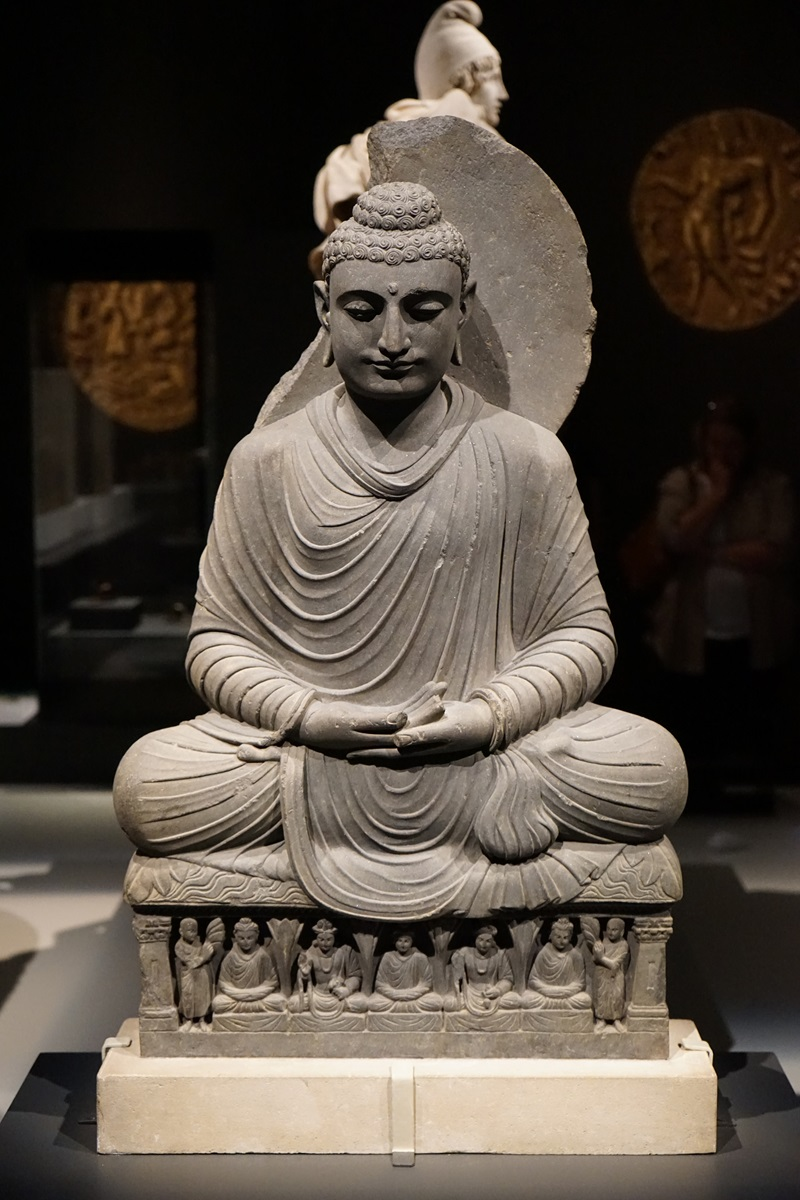
\includegraphics[width=\linewidth]{buddhism.jpg}
    \caption{Four Noble Truths - World History Encyclopedia}
\end{figure}
\end{column}
\end{columns}
\end{frame}

%%%%%%%%%%%%%%%%%%%%%%%%%%%%%%%%%%%%%%%%%%%%%%%%%%%%%%%%%%%%%%%%%%%%%%%%%%%%%%%%%%
\begin{frame}[fragile]\frametitle{Jainism}
\begin{columns}
\begin{column}{0.5\textwidth}
\begin{itemize}
    \item Jainism is an ancient Indian religion that emphasizes non-violence (ahimsa)
    \item Believes in the existence of multiple, eternal, and uncreated universes
    \item Promotes the concept of karma and the cycle of birth, death, and rebirth
    \item Adherents follow strict vows, including non-violence, truthfulness, and non-stealing
    \item Jain scriptures include the Agamas and the Puranas
\end{itemize}
\end{column}
\begin{column}{0.5\textwidth}
\begin{figure}
    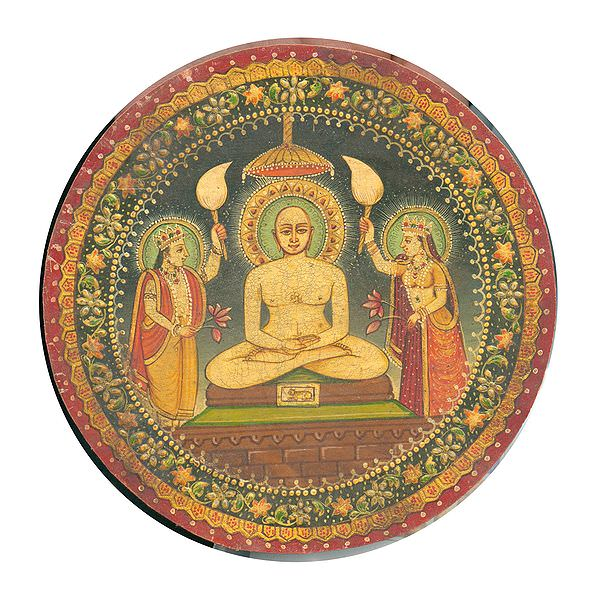
\includegraphics[width=\linewidth]{jainism.jpg}
    \caption{Jainism - World History Encyclopedia}
\end{figure}
\end{column}
\end{columns}
\end{frame}

%%%%%%%%%%%%%%%%%%%%%%%%%%%%%%%%%%%%%%%%%%%%%%%%%%%%%%%%%%%%%%%%%%%%%%%%%%%%%%%%%%
\begin{frame}[fragile]\frametitle{Sikhism}
\begin{columns}
\begin{column}{0.5\textwidth}
\begin{itemize}
    \item Sikhism is a monotheistic religion founded by Guru Nanak in the 15th century
    \item Believes in the concept of Ik Onkar, the one supreme, formless God
    \item Emphasizes the importance of equality, service, and social justice
    \item Sikhs follow the teachings of the ten Sikh Gurus and the Sikh scriptures
    \item Promotes the practice of Naam Simran (meditation on the divine name)
\end{itemize}
\end{column}
\begin{column}{0.5\textwidth}
\begin{figure}
    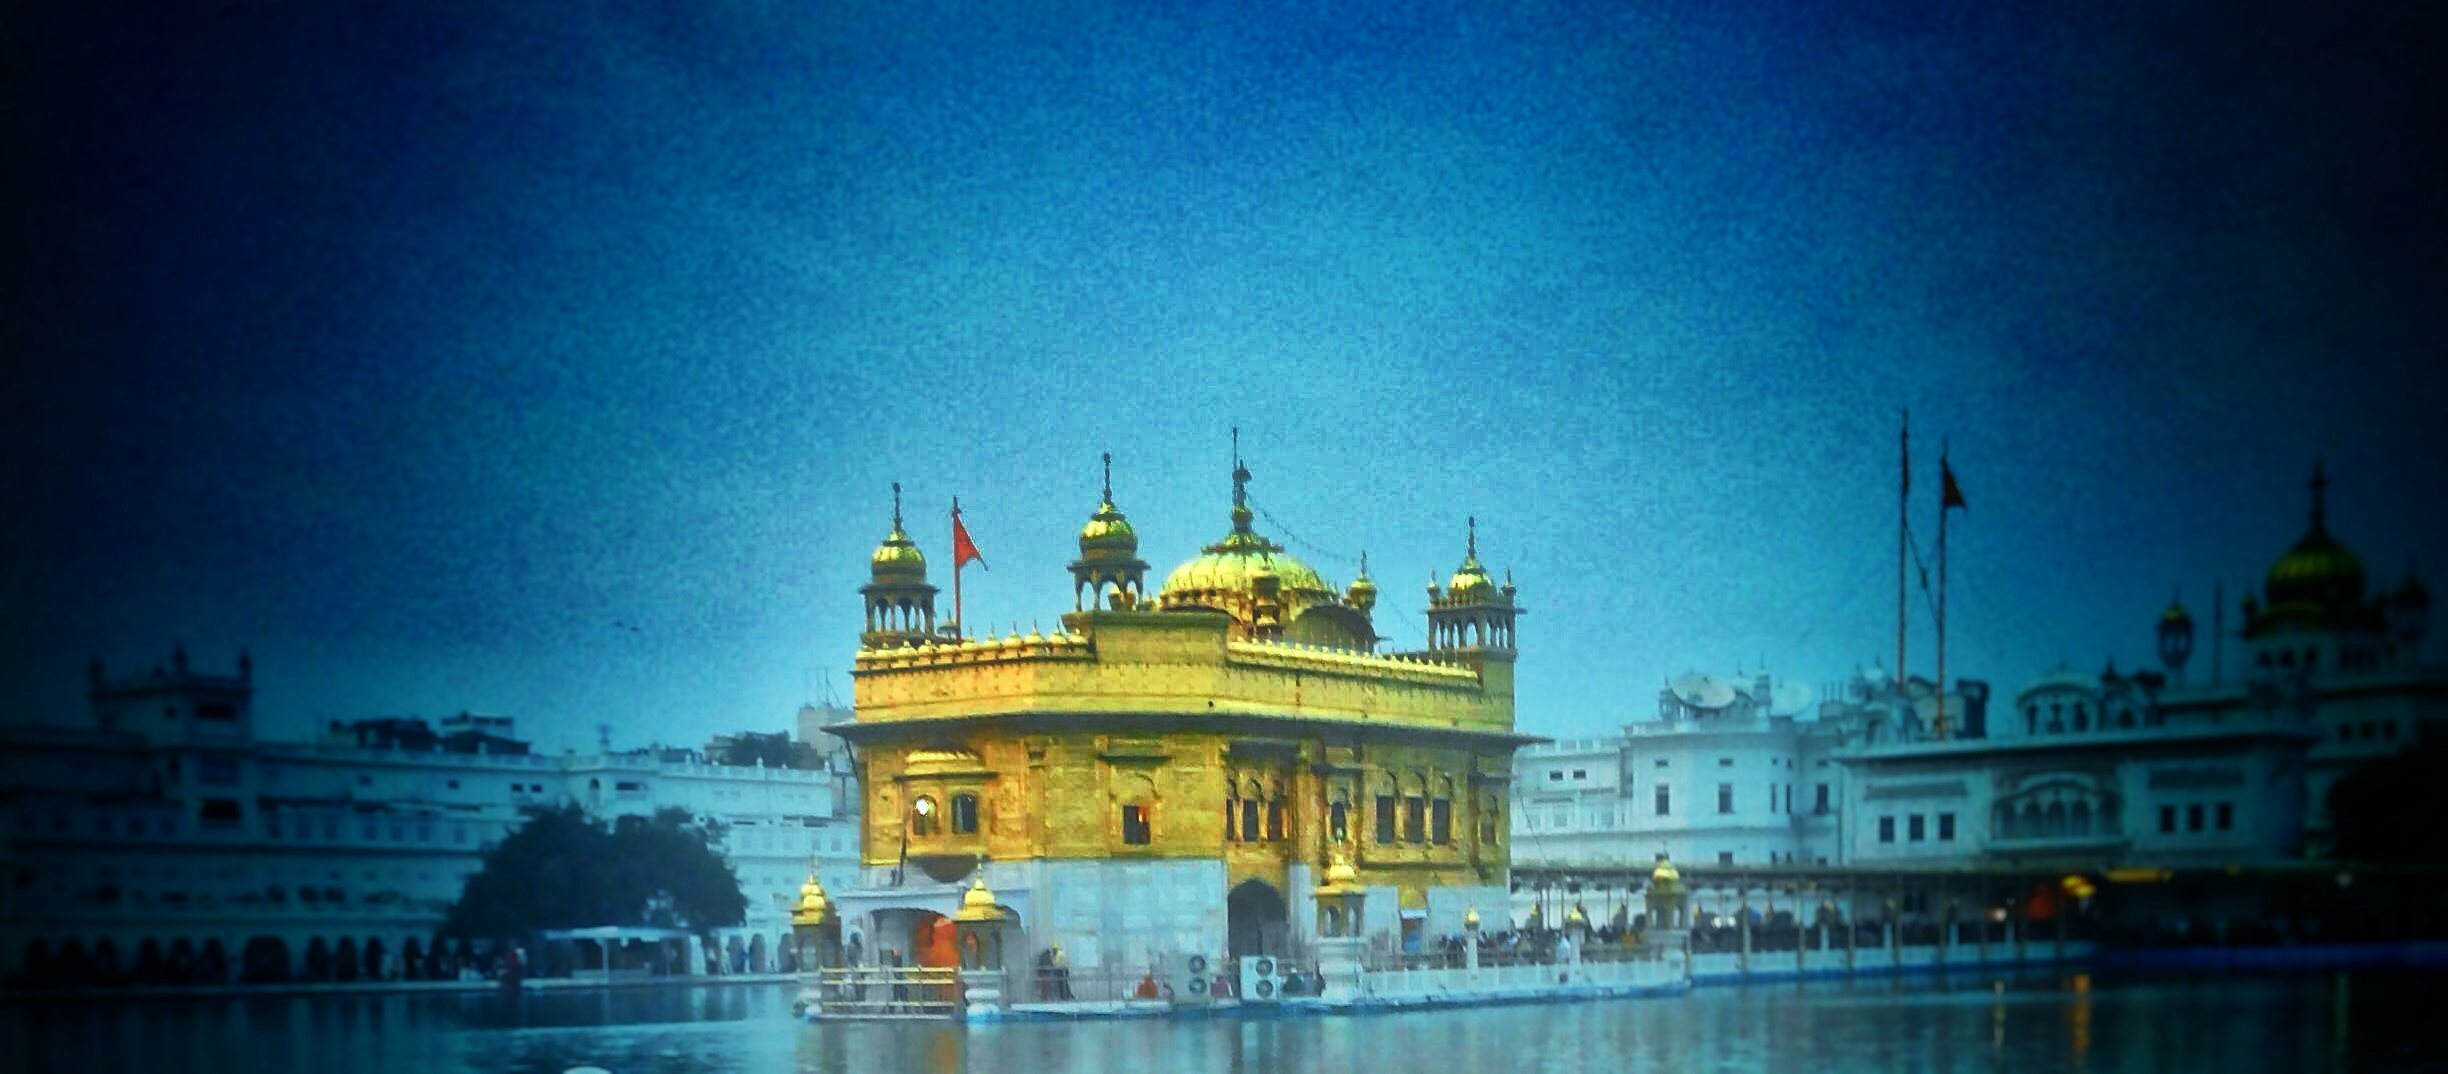
\includegraphics[width=\linewidth]{sikhism.jpg}
    \caption{Golden Temple Sikhism - Wikimedia Commons}
\end{figure}
\end{column}
\end{columns}
\end{frame}